% Copyright (c) 2008-2009 solvethis
% Copyright (c) 2010-2011 Casper Ti. Vector
% Public domain.

\chapter{验证平台设计与实现}\label{chap:implementation}
	本章介绍支持物理层WiFi安全研究的验证平台的设计与实现。
	在\ref{sec:grt2.0_design}节将介绍本研究的前期工作GRT2.0系统,
	GRT系统是本课题组提出的一款高性能可重构的软件无线电通信平台\cite{pkuraw},
	GRT2.0系统是其最新的发布版本,应用有全双工\cite{mna16grt}、认知无线电\cite{fpga17grt}、低延迟通信等。
	在\ref{sec:grtsec_design}节将介绍本研究为了支持物理层WiFi安全研究,
	在GRT2.0上进行的改进和扩展,称作GRTSEC,重点是物理层信息的提取、分析框架。

	\section{GRT2.0系统介绍}\label{sec:grt2.0_design}
		GRT2.0系统是本组合作完成的项目,旨在帮助无线通信的软硬件研究与开发人员
		更好更快地在真实的通信系统中实现和验证无线通信系统物理层和MAC层的算法,
		本人负责其中射频通信库和工程自动化脚本,参与了LOW MAC模块的搭建。
		本节将对整体进行简单介绍,对本人完成或参与的部分进行具体展开。
		在\ref{subsec:grt2.0_overview}小节介绍GRT2.0系统的整体框架,
		在\ref{subsec:grt2.0_rfd}小节介绍射频通信库的设计,
		在\ref{subsec:grt2.0_script}小节介绍工程自动化脚本,
		在\ref{subsec:grt2.0_drawback}小节分析GRT2.0系统用于物理层WiFi安全研究时的不足,
		在\ref{subsec:grt2.0_summary}小节对本节进行简单总结。

		\subsection{GRT2.0整体框架介绍}\label{subsec:grt2.0_overview}
		在硬件组成上,GRT2.0系统包括四个部分,FPGA、上位主机、FPGA配置计算机、射频前端,
		如图\ref{fig:grt_overview}所示,
		其中上位主机与FPGA配置计算机可以是同一台计算机,各部分介绍如下:
			\begin{itemize}
				\item FPGA:作为无线电通信平台的核心数据处理硬件,包括射频通信库、物理层模块、LOW MAC模块、USB通信库四个部分,
				射频通信库负责射频前端的交互,
				物理层模块实现了802.11规定的物理层全部的数据处理过程,
				LOW MAC模块实现了802.11规定的MAC层的时序要求高的数据处理过程和控制流程,
				USB通信库负责与上位计算机的交互。
				\item 上位主机:运行GRT2.0的驱动,与上层网络协议栈连接,运行应用程序。
				\item FPGA配置计算机:FPGA的开发、烧写与调试。
				\item 射频前端:负责射频通信。
			\end{itemize}

			\begin{figure}
				\centering
				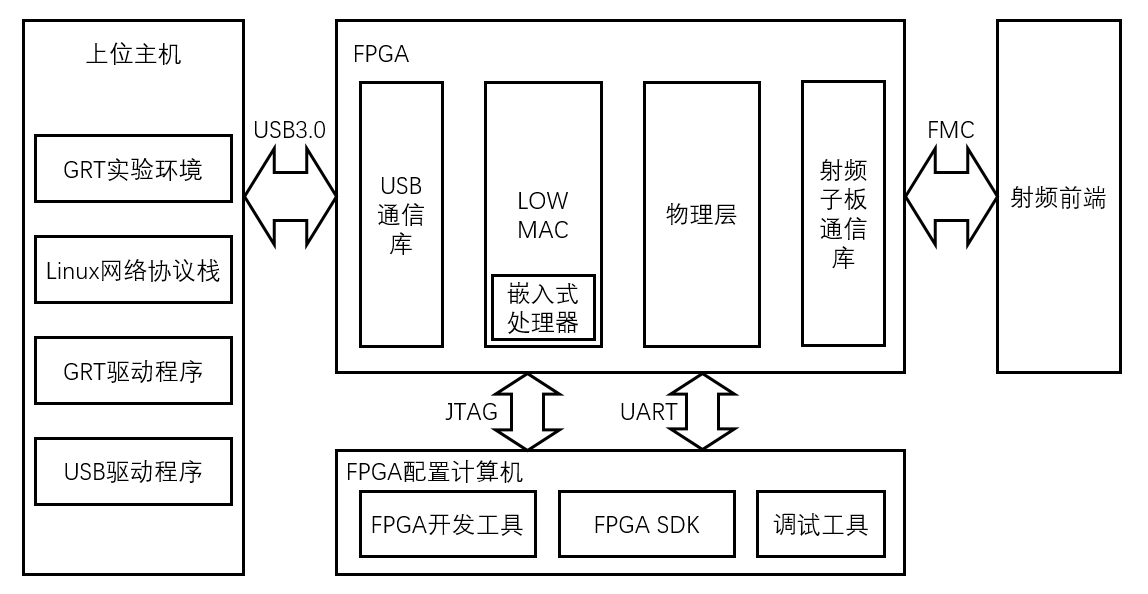
\includegraphics[width=1.0\textwidth]{img/GRT_overview.png}
				\caption{GRT2.0整体结构示意图}
				\label{fig:grt_overview}
			\end{figure}
		目前GRT2.0系统的FPGA部分使用的是Xilinx KC705开发板,后续版本也对Xilinx VC707进行了支持,
		上位主机使用的操作系统是Ubuntu14.04,
		FPGA配置计算机使用的开发工具是Vivado2015.2及其对应版本的SDK,
		射频前端使用的是Analog Device公司的EVAL-AD-FMCOMMS3-EBZ开发板\cite{fmcomms3}。

		值得一提的是,FPGA上的LOW MAC模块采用了软硬件协作的结构,
		将嵌入式处理器MicroBlaze\cite{microblaze}与硬件IP核\cite{xilinxip}结合,
		图\ref{fig:grt_lowmac}是LOW MAC模块软硬件协作的结构示意图,我参与了LOW MAC模块的搭建。
		硬件IP核是对完成特定功能的硬件逻辑的封装,
		嵌入式软件与硬件IP核结合的方式可以大大提高系统编程的灵活性。
		流程控制在嵌入式软件中实现,例如根据一帧的MAC地址进行分支处理,
		如果由硬件实现会非常繁琐,可读性和可扩展性差,
		数据通路和密集计算在硬件IP核中实现,例如发送端增加CRC校验位、接收端检测CRC是否匹配,
		硬件IP核可以每个时钟周期计算64bit的CRC,
		如果由软件实现会造成很高的延迟。
		在Vivado开发套件中,嵌入式处理器MicroBlaze与硬件IP核共同组织成Block Design\cite{xilinxblockdesign}的形式,具有图形化的开发界面。
		为了提高可编程性,我在射频通信库设计与GRTSEC的设计中,也加入了软硬件协作的结构,
		在\ref{subsec:grt2.0_rfd}小节和\ref{sec:grtsec_design}会进行进一步介绍。

			\begin{figure}
				\centering
				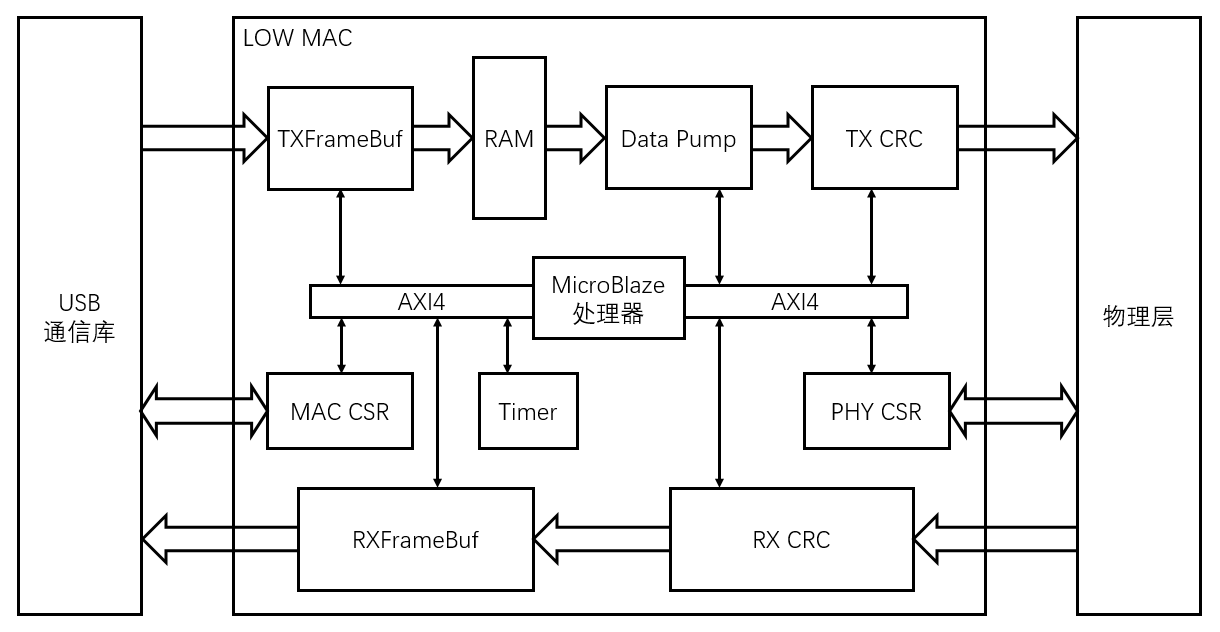
\includegraphics[width=1.0\textwidth]{img/GRT_lowmac.png}
				\caption{LOW MAC模块软硬件协同结构示意图}
				\label{fig:grt_lowmac}
			\end{figure}

		\subsection{射频通信库}\label{subsec:grt2.0_rfd}
		射频前端是无线开放平台必备的组成部分,负责将数字基带信号转变为射频信号发送到空气中,
		以及接受空气中的射频信号转变为数字基带信号,射频前端的通信性能决定了无线平台的适用场景,
		对于WiFi无线验证平台,需要一个支持2.4GHz和5GHz中心频点、40MHz带宽的射频前端。
		作为一个提供给研究者的开放平台,除了考虑通信性能外,还要考虑价格,
		价格过高会让研究者望而却步。例如,OpenMili平台使用的射频前端\cite{mobicom16openmili}价格约11000美元,用于无线研究时价格过高。

		在GRT1.0系统中,我们选择使用USRP N210搭配XCVR2450子板\cite{usrpn210}作为射频前端,
		USRP N210价格是17000元,XCVR2450子板价格是4000元,属于可接受的范围。
		USRP的驱动是运行在Linux操作系统上的,称作UHD(USRP Hardware Driver),
		为了将FPGA开发板与射频前端相连,我们在FPGA上实现了USRP的硬件驱动,作为GRT1.0的射频通信库。
		这样的方式有以下几个缺点:
			\begin{itemize}
				\item XCVR2450子板最高支持25MHz带宽,无法达到802.11n协议要求的40MHz;
				\item USRP N210与FPGA开发板通过千兆以太网接口相连,
				以太网协议栈引入了不必要的延迟,经过GRT1.0射频通信库优化后的延迟也高达30ms以上,
				超过了802.11协议中要求的18ms的回复ACK的间隔,
				虽然可以与某些延迟要求宽松的商用设备实时通信,但系统的扩展性变得很差;
				\item 硬件实现USRP驱动的过程复杂,无法利用官方提供的软件驱动程序,也不方便驱动程序的升级换代;
				\item 不支持多天线MIMO(Multiple Input Multiple Output),MIMO技术是802.11n协议要求的技术;
			\end{itemize}

		以上缺点制约了无线平台的应用范围。

		在GRT2.0中,经过多方比较,我们选择使用性能更好、支持2x2 MIMO、具有通用接口的射频前端,
		Analog Device公司的EVAL-AD-FMCOMMS3-EBZ射频开发板\cite{fmcomms3},简称FMCOMMS3。
		FMCOMMS3的价格为6200元,射频芯片为Analog Device公司的AD9361,
		支持的中心频率范围是70MHz至6GHz,可以覆盖WiFi使用的2.4GHz和5GHz频段,
		带宽为200kHz至56MHz可调,支持802.11a协议要求的20MHz带宽、
		802.11b协议要求的18MHz带宽和802.11n协议要求的40MHz带宽,支持2x2 MIMO,
		通过高带宽的FMC接口(FPGA Mezzanine Card)\cite{wikifmc}与FPGA相连。
		虽然生产商提供了FPGA参考设计,但仍然无法直接与GRT系统集成,例如占用了过多的FPGA资源,没有提供上位主机配置射频参数的接口。
		射频通信库完成了GRT2.0系统与FMCOMMS3射频子板的对接。

		GRT2.0射频通信库的设计采用了嵌入式处理器与硬件IP核结合的方式。
		射频通信库软件部分所做的工作主要是对配置射频参数的接口进行封装,
		通过USB通信库与上位主机的驱动程序连接起来。
		由主机驱动程序配置的射频参数有中心频率和带宽,由射频通信库软件接口提供给主机驱动程序的是RSSI。

		射频通信库硬件部分对生产商提供的参考设计进行了较大的改造,体现在以下几点:
			\begin{itemize}
				\item 参考设计通过以太网与主机相连,通过HDMI与显示器相连,
				为降低FPGA资源使用率,射频通信库硬件部分去除对多种冗余接口的控制器,包括与主机相连的以太网接口控制器和以太网DMA控制器,
				与显示器相连的HDMI接口控制器,与板上LCD显示屏相连的LCD控制器,IIC接口控制器,只保留与FMC子板相连的FMC接口控制器;
				\item 参考设计将主机通过以太网发来的数据DMA到DDR3中,然后从DDR3中读取数据,
				经过AD9361 IP核转为时钟对齐的IQ两路数据,发送给FMCOMMS3子板,接收端与之方向相反,
				为降低数据传输延迟,射频通信库硬件部分去除收发数据读写DDR3的过程,直接转为FIFO接口与GRT系统的物理层模块相连;
				\item 参考设计中MicroBlaze配置级别高,性能好,
				为降低MicroBlaze占用的FPGA资源,射频通信库硬件部分简化了MicroBlaze的配置,
				提供支持射频通信库软件部分和LOW MAC软件部分的最小集合。
			\end{itemize}

		下面分别介绍射频通信库的数据通路的硬件接口和配置的嵌入式软件接口。
		在硬件设计中,射频通信库将AD9361 IP核输出的IQ两路数据转化为标准的FIFO接口,提供给物理层,并通过异步FIFO的方式完成时钟域转换。
		射频侧的时钟和复位信号由AD9361 IP核提供,这个时钟是随采样率变化的;物理层侧的时钟和复位信号由物理层提供。
		硬件接口以简单明了为目标,
		射频通信库与物理层之间的接口定义如下:
		\begin{lstlisting}[language={Verilog}]
module fmc_iface #(
	parameter integer MODE = RFD_MODE_RF
)
(
	input fmc_clk,
	input fmc_rst,
	input PHY_TX_clk,
	input PHY_RX_clk,
	input PHY_rst,
	output PHY2RF_FIFO_prog_full,
	input PHY2RF_FIFO_wr_en,
	input [31:0] PHY2RF_FIFO_din,
	input RF2PHY_FIFO_rd_en,
	output [31:0] RF2PHY_FIFO_dout,
	output RF2PHY_FIFO_empty,
	output RF2PHY_FIFO_almost_empty
);
		\end{lstlisting}

		射频通信库在嵌入式软件端提供了配置射频参数接口。
		包括初始化射频子板,对射频子板的ADC、DAC、滤波器等初始化配置,设置中心频率、采样率、发送增益等射频参数。
		中心频率的单位是MHz,比如WiFi标准频段的信道1为2412MHz。
		采样率的单位为Sps(Samples per seconds),比如802.11a/g的采样率为20000000Sps,802.11n需要40000000Sps的模式。
		发送增益以衰减的形式表示,单位是mdb,即db的千分之一,设置为0时表示无衰减,1000时为衰减为十分之一。
		射频通信库提供的软件配置接口如下:
		\begin{lstlisting}[language={C}]
int fmc_main(void);
void set_rx_samp_freq(double* param, char param_no);
void set_tx_samp_freq(double* param, char param_no);
void set_rx_lo_freq(double* param, char param_no);
void set_tx_lo_freq(double* param, char param_no);
void set_tx1_attenuation(double* param, char param_no);
		\end{lstlisting}

		\subsection{工程自动化脚本}\label{subsec:grt2.0_script}
		TCL脚本在FPGA的开发过程中有着广泛的运用\cite{xilinxtcl},从模块间引脚的连接、工程文件的组织,
		到调试信息的导出、自动执行工作流程,TCL脚本大大提高了FPGA开发的效率。
		为了将GRT2.0系统开源给研究者,我们提供了可以自动搭建工程项目的TCL脚本,
		实现了从源代码、资源文件到最终二进制文件的自动化过程。
		TCL脚本的使用是从GRT1.0到GRT2.0的一个重要改进。

		GRT2.0系统提供的工程自动化TCL脚本完成了以下过程:
			\begin{itemize}
				\item 对GRT2.0提供的完成特定功能的硬件逻辑封装成IP核\cite{xilinxip};
				\item 生成Block Design\cite{xilinxblockdesign}中的各个模块和输入输出端口,完成模块间、端口间互相的连线;
				\item 生成和配置嵌入式处理器MicroBlaze\cite{microblaze}及其附属的总线控制器,对总线地址进行分配;
				\item 对Xilinx提供的IP核进行配置,并添加到工程中,主要是各种不同类型的FIFO、时钟生成器、RAM、DDR3控制器等;
				\item 添加GRT2.0的资源文件,有约束文件、三角函数数据文件、OFDM导频数据文件等;
				\item 执行工作流程,设置流程策略,工作流程有综合(Synthesis)、布局(Place)、布线(Route)、生成二进制文件(Generate Bitstream)等;
			\end{itemize}

		通过执行工程自动化TCL脚本,用户可以利用手中的开发板和开源的GRT2.0代码,生成可以烧写FPGA的二进制文件,
		再结合我们提供的上位主机的驱动程序,用户便自行搭建GRT2.0系统完成。

		\subsection{用于安全研究时的不足}\label{subsec:grt2.0_drawback}
		基于GRT2.0系统进行开发,可以满足设计目标中的与商用网卡实时通信,以及与上层网络协议栈连接,
		但在其他方面存在不足,尤其是无法获取物理层WiFi安全研究所需要的物理层信息。
		GRT2.0系统中物理层接收端的设计目标是消除接收信号的偏差,还原出发送信号,
		频偏纠正、相位纠正、信道均衡、Viterbi解码等过程都是为了完成这个目标,
		然而在物理层WiFi安全的研究中,接收信号的偏差有其背后的物理含义,常常被拿来做研究,
		但GRT2.0的系统框架不支持这些信息的提取。
		具体来说,用于安全研究时的不足包括以下几点。
			\begin{itemize}
				\item 物理层由单一的硬件逻辑实现,可编程性还不够高;
				\item 未提供方便获取CSI、RSSI的接口,CSI和RSSI是安全研究常用的指标;
				\item 在接收端数据处理过程中消除了信号偏差,而这些偏差在安全研究中常常被用到,例如频偏;
				\item 不支持软硬件数据处理模块替换的能力;
				\item 缺乏物理层编程的使用样例;
			\end{itemize}

		在下一节\ref{sec:grtsec_design},将针对以上问题加以改进,
		介绍适用于物理层WiFi安全研究的验证平台GRTSEC的设计与实现。

		\subsection{本节小结}\label{subsec:grt2.0_summary}
		本节对支持物理层WiFi安全研究的验证平台GRTSEC的前期工作GRT2.0系统进行了介绍,
		GRT2.0系统硬件上包括上位主机、FPGA、射频前端、配置计算机,
		由物理层模块、LOW MAC模块、射频通信库、USB通信库等模块组成。
		GRT2.0系统可以满足本文设计目标中的与商用网卡实时通信,以及与上层网络协议栈连接,
		但在获取物理层信息、物理层编程性、软硬件模块替换等方面不满足设计目标。
		另外,本节展开介绍了我在GRT2.0系统中完成的工作,主要负责完成的射频通信库、工程自动化脚本,
		参与完成的LOW MAC软硬件协作设计。

	\section{GRTSEC设计与实现}\label{sec:grtsec_design}
		在本节将介绍GRTSEC在GRT2.0系统上的改进,
		\ref{subsec:grtsec_overview}小节对总体设计和设计思路进行介绍,
		GRTSEC最核心的改进是对物理层信息进行了支持,提取了物理层信息并提供了物理层信息的编程接口,
		\ref{subsec:grtsec_phyinfo_substract}小节介绍物理层信息的提取方法,
		\ref{subsec:grtsec_phyinfo_api}小节介绍物理层信息的软件编程接口,
		\ref{subsec:grtsec_phyinfo_analyzer}小节介绍用于做物理层信息分析的硬件模块设计,
		\ref{subsec:grtsec_phyinfo_extension}小节介绍用户如何得到自定义的物理层信息,
		\ref{subsec:grtsec_loopback}小节介绍为提高开发调试的效率,射频通信库模块做的改进。

		\subsection{总体设计}\label{subsec:grtsec_overview}
		针对物理层WiFi安全研究,GRTSEC在GRT2.0的基础上的改进主要体现在三方面,
		一是扩展了软硬件协同工作的范围,将物理层也与嵌入式处理器通过总线相连,
		方便用户直接对物理层进行配置,以及从物理层获取数据;
		二是提取了常用的物理层信息并提供给用户软硬件的编程接口;
		三是设计了对物理层信息进行分析的软件代码和硬件模块。

		GRTSEC的硬件结构如图\ref{fig:grtsec_hw_design},
		图中block design内为软硬件协同设计的部分,由于暂未有对USB通信库编程的需求,放在block design之外,
		图中Core为原GRT2.0中的嵌入式MicroBlaze处理器,
		Low mac TX、Low mac RX为原GRT2.0中LOW MAC模块的发送端和接收端部分,
		以上为保留的GRT2.0的设计。
		图中PHY TX和PHY RX是将原先的物理层模块移入block design中,与嵌入式处理器通过AXI总线相连,
		射频通信库也移入block design中,
		图中PHY Analyzer模式是GRTSEC新增加的硬件IP,用于对从物理层模块得到的物理层信息进行数据分析,
		并将分析结果反馈给嵌入式软件。
			\begin{figure}
				\centering
				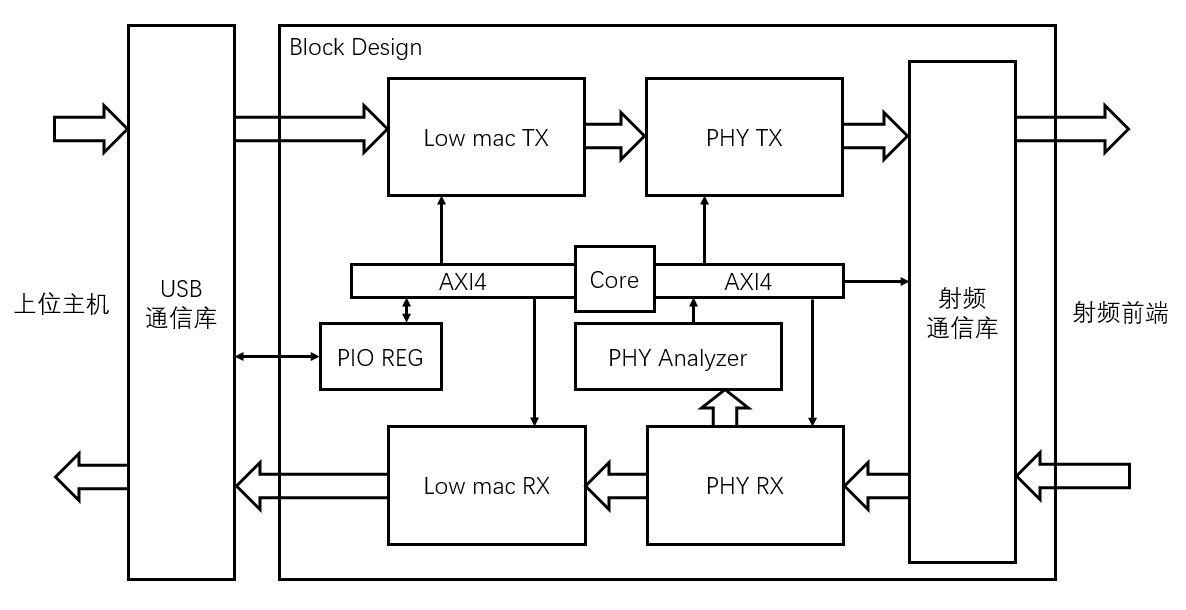
\includegraphics[width=1.0\textwidth]{img/GRTSEC_hw_design.png}
				\caption{GRTSEC硬件模块设计图}
				\label{fig:grtsec_hw_design}
			\end{figure}


		\subsection{常用物理层信息的提取}\label{subsec:grtsec_phyinfo_substract}
		在实际的物理层信息提取过程中,我们对物理层信息进行分类,
		第一类是随帧物理层信息,每一帧包含一组值,通过前导码(preamble)计算得到,比如CSI、频偏、RSSI、调制方式,
		第二类是随符号物理层信息,每一个符号(symbol)包含一组值,每一帧有多个符号,最典型的是导频,
		第三类是随采样点物理层信息,每个采样点有一个值,比如星座点偏移向量。
		在物理层WiFi安全的研究中,绝大多数使用的是第一类,随帧物理层信息,GRTSEC对这一类物理层信息进行了提取。
		GRTSEC虽然未提供随符号物理层信息和随采样点物理层信息的接口,但在各个模块中包含有原始信息,用户可自行提取,
		参照\ref{subsec:grtsec_phyinfo_extension}小节进行扩展。

		对于随帧物理层信息的提取,需要解决两个问题,一是物理层信息的帧对齐问题,二是精确接收时间问题。
		物理层信息的帧对齐问题是指当软件MAC层收到一帧时,如何获取该帧对应的物理层信息,
		假如此时去物理层取,有可能下一帧已经到来,得到的是下一帧的信息,也有可能当前帧的物理层信息尚未计算完毕,得到的是上一帧的信息。
		精确接收时间问题是指软件MAC层收到一帧时如何知道该帧的精确到来时间,
		在TMC 10\cite{tmc10clock}这篇文章中提出利用帧到来时间作为计算硬件指纹的依据,到来时间必须精确到us级别,
		但软件代码的执行会受操作系统调度的影响,即使是嵌入式软件,也会受中断的影响,无法精确的标定帧到来的时间。

		对于物理层信息的帧对齐问题,我们采用三级缓存的方法。
		当物理层收到一帧,各个模块通过前导码计算得到物理层信息后,保存在模块内部,与模块的时钟对齐,称作模块内缓存。
		SIGNAL字段在前导码的后面,当此帧的SIGNAL字段被正确解出,且LOW MAC准备好接收下一帧时,物理层会通知LOW MAC模块收到了一帧,
		向嵌入式处理器发起一次中断,此时,我们将模块内缓存的物理层信息,经过时钟域转换,在另一组统一时钟的寄存器中缓存,称作物理层缓存,
		这一步的目的是让各个模块可以继续处理下一帧,更新模块内缓存。
		LOW MAC的软件收到中断后,将物理层缓存的物理层信息,存放到与AXI总线时钟对齐的第三组寄存器中,称作AXI缓存,
		处理器通过AXI总线读取AXI缓存的物理层信息,此时读到的即为收到中断的那一帧的物理层信息,
		这一步的目的是让物理层可以向LOW MAC发起下一帧的终端,而嵌入式处理器在一帧之内的后面的任意位置都可以读取这一帧的物理层信息。
		我们将物理层信息缓存在寄存器中,而不是将物理层信息缓存在队列中,因为SIGNAL有可能会解错,嵌入式软件也可能会丢掉中断,
		一旦SIGNAL错误或中断没有被处理,缓存的物理层信息就不会继续被读取,阻塞了队列,队列发生错位。
		假如缓存在寄存器中,发生错误时后面帧的物理层信息会覆盖前面的,不会引起错位。
		图\ref{fig:phy_info_cache}描述了三级缓存的思想。
			\begin{figure}
				\centering
				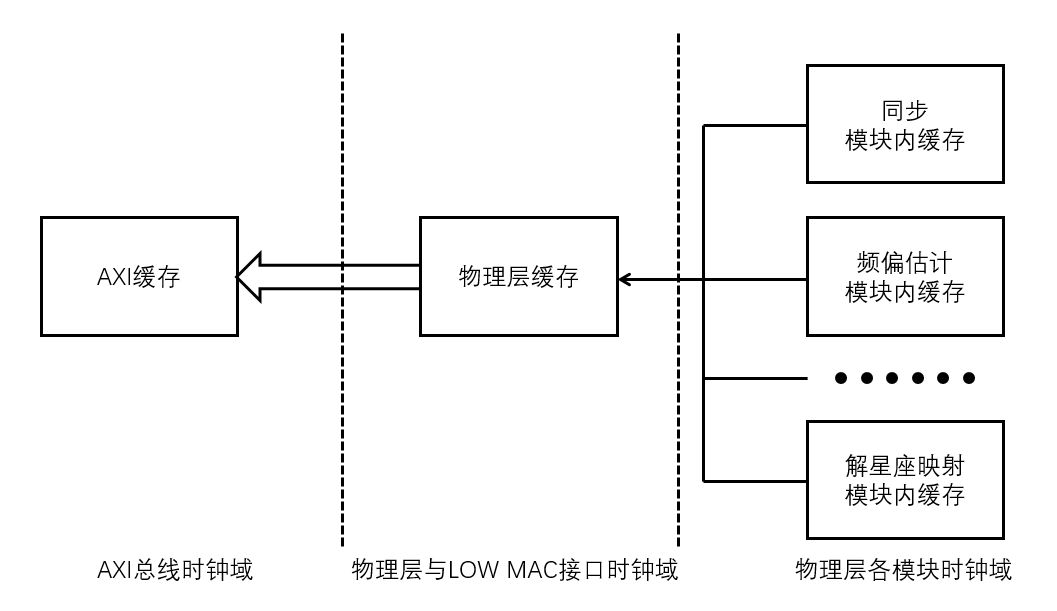
\includegraphics[width=0.7\textwidth]{img/phy_info_cache.png}
				\caption{GRTSEC物理层信息三级缓存示意图}
				\label{fig:phy_info_cache}
			\end{figure}

		对于精确接收问题,GRTSEC采用物理层时间戳的方法。首先,我们在物理层与LOW MAC接口处使用一个64位的计数器,每一个时钟周期加一,
		目前此处的时钟频率是100MHz,那么计数器的精度就是10ns。然后,当物理层同步到一帧时,读取计数器的值并保持下来,
		LOW MAC软件通过AXI总线读取保存的计数器值。这种方法是把计数器的值也当做一种物理层信息,采用三级缓存技术进行记录,计数器相当于模块内缓存。
		AXI总线一次读写的宽度是32位,一般而言,读取计数器的低32位寄存器即可,低32位可以记录约43秒的时间间隔,对于超过43秒的时间,则读取高32位寄存器。

		接下来介绍几种常用随帧物理层信息的提取方法,具体来说,包括CSI、频偏、RSSI、调制方式。
		在第三章需求分析中我们提到,CSI和RSSI是安全研究中最常用的的物理层信息,频偏在基于身份验证的安全机制中也常常被用到。
		调制方式是指物理层数据处理过程中的信源调制方式,对于802.11协议,调制方式有BPSK、QPSK等,
		调制方式是物理层信息的重要参考,提取方式较为简单,分析物理层帧结构,从信令字段(SIGNAL)可以直接得到。
		而RSSI可以通过FMCOMMS3子板的嵌入式驱动程序得到,我们不需要进行提取,直接提供编程接口。
		以下将分别对CSI和频偏的提取过程进行介绍。

			\begin{figure}
				\centering
				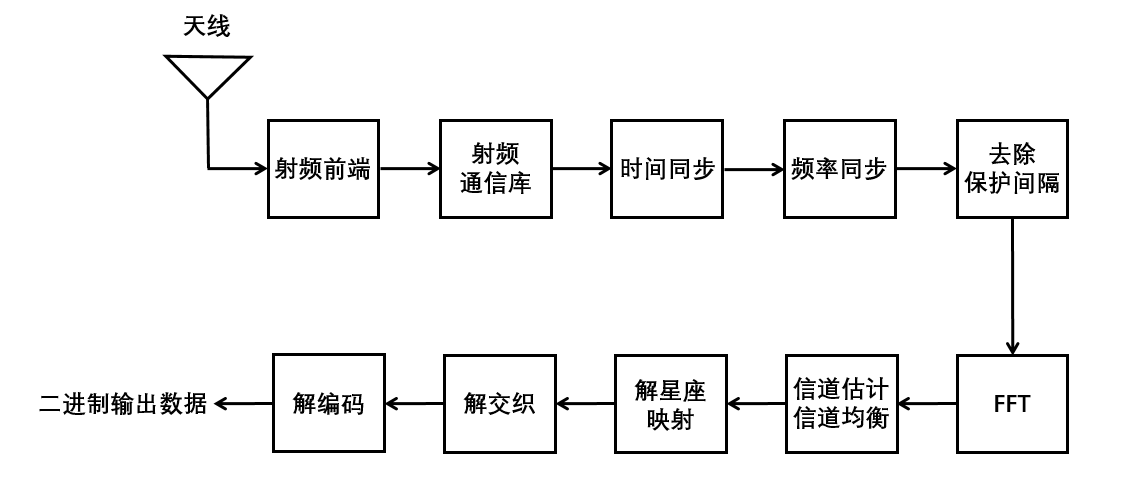
\includegraphics[width=0.8\textwidth]{img/GRT_phy_rx.png}
				\caption{GRTSEC物理层接收端模块示意图}
				\label{fig:GRT_phy_rx}
			\end{figure}

		首先介绍CSI。作为OFDM通信系统,802.11的CSI是指各个子载波当前的信道状况。
		我们假设在一帧的接收过程之内,CSI大致不变,802.11协议也是基于此假设使用训练字段对信道进行估计。
		GRTSEC的物理层接收端模块示意图见\ref{fig:GRT_phy_rx},我们在信道估计模块提取到CSI。
		图\ref{fig:80211_spec_preamble}介绍了802.11a/g物理层训练字段的结构,
		训练字段是发送端发送一段双方已知的序列,接收端根据接收序列来做同步、信道估计等。
		802.11a/g物理层帧结构规定了两个训练字段,先是160个采样点的短训练字,后是160个采样点的长训练字,
		在长训练字后面是80个采样点的SIGNAL字段,里面规定了帧长度和调制方式。
		短训练字以16个采样点为周期,共10个周期,采样点间隔为0.05$us$,用来做AGC(自动增益控制)、时间同步、频率同步等,
		在后面介绍提取频偏和RSSI时会进一步说明。
		长训练字前32个采样点是保护间隔,抽取$T_1$、$T_2$各16个采样点组成的,
		$T_1$、$T_2$是重复的。长训练字用来做信道估计、细粒度的频偏估计。
			\begin{figure}
				\centering
				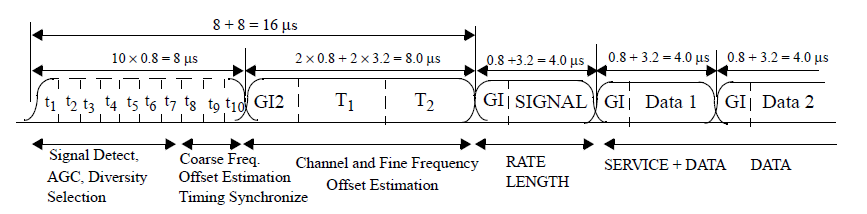
\includegraphics[width=1.0\textwidth]{img/80211_spec_preamble.png}
				\caption{802.11前导码结构}
				\label{fig:80211_spec_preamble}
				\cite{ieee80211}
			\end{figure}

		我们从长训练字中提取CSI。长训练字的采样点为1与-1的序列,如式\ref{fig:80211_lts_sequence},不包含其他值(中间的0为直流分量,不承载信息),
		因此接收值只需转换符号即可得到各个子载波的信道状况。而短训练字中除了1与-1外,还有0和1+j这样的值,不适合提取CSI。
		具体实现时,我们预存长训练字的理论值,与接收到的长训练字进行比较,理论值为-1时对接收值转换符号,理论值为1时不变。
		符号转换后得到52个采样值组成的向量,这个向量便可以代表此帧的CSI。

			\begin{figure}
				\centering
				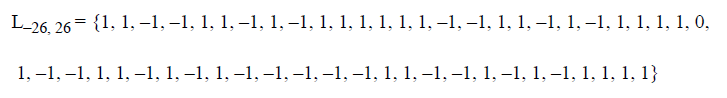
\includegraphics[width=0.9\textwidth]{img/80211_lts_sequence.png}
				\caption{802.11前导码长训练字采样值}
				\label{fig:80211_lts_sequence}
				\cite{ieee80211}
			\end{figure}

		然后介绍频偏的提取。频偏在频偏估计模块中提取,利用短训练字的周期性,具体来说,
		使用短训练字的后64个采样点,即10个周期中的后4个周期,原因有两点,
		一是前面的采样点会受AGC(Automatic Gain Control,自动增益控制)的影响,幅度有波动,
		二是大多数时候从短训练字的中间位置同步到一帧,前面部门有可能同步不到,而后4个周期实践表明是切实可行的。
		我们首先对频偏公式进行变换,此处的推导比第二章更加详细,并结合具体实现。
		假设$k_1$、$k_2$时刻的接收值为$r(k_1)$和$r(k_2)$,理论值为$s(k_1)$和$s(k_2)$,有以下公式:
			\begin{equation}
				\centering
				r(k_1)=s(k_1) \cdot e^{j2 \pi \Delta fk_1 / f_s}
				\label{fig:freq_offseet_rs_1}
			\end{equation}
			\begin{equation}
				\centering
				r(k_2)=s(k_2) \cdot e^{j2 \pi \Delta fk_2 / f_s}
				\label{fig:freq_offseet_rs_2}
			\end{equation}

		其中,$\Delta f$为要求的频偏,$f_s$为采样频率,在802.11a/g中数值为20M,在802.11n中有20M和40M两种情况。
		$r(k_1)$、$r(k_2)$、$s(k_1)$、$s(k_2)$、$f_s$均已知,我们可以通过以下方式求出。
		根据短训练字每16个采样点重复一次的特性可知,当$k_2 = k_1 + 16$时,$s(k_1) = s(k_2)$,
		代入前面的公式,可以推出以下两式:
			\begin{equation}
				\centering
				def: \frac{r(k_1)}{r(k_2)} = A + Bj
				\label{fig:freq_offseet_AB_def}
			\end{equation}
			\begin{equation}
				\centering
				\Delta f = \frac{f_s}{2\pi \cdot 16} \cdot arctan(\frac{B}{A})
				\label{fig:freq_offseet_result}
			\end{equation}

		式\ref{fig:freq_offseet_AB_def}由复数的性质推出,$r(k_1)$、$r(k_2)$都是复数,相除的结果也是复数,
		复数总是可以写成$A + Bj$的形式,其中$A$、$B$为实数。
		式\ref{fig:freq_offseet_result}是将式\ref{fig:freq_offseet_AB_def}代入
		式\ref{fig:freq_offseet_rs_1}、\ref{fig:freq_offseet_rs_2}得出,得到频偏值。

		在具体实现时,我们在硬件中得到$A$、$B$,作为物理层信息传给软件,再由软件计算$arctan$和常数乘法得到频偏。
		硬件计算$A$、$B$时,需要对每隔16个的接收采样点进行相除,
		复数相除$\frac{r(k_1)}{r(k_2)}$可以转化为$\frac{1}{|r(k_2)|^2}r(k_1) \cdot r(k_2)^* $。
		每一个采样点都可以跟它之前的第16个采样点得到一组$A$、$B$,我们对64个采样点得到的64个$A$、$B$进行相加求平均,降低误差,
		最终提取到的物理层信息即为平均的$A$、$B$,分别代表周期性偏移实部和周期性偏移虚部。

		\subsection{物理层信息软件编程接口}\label{subsec:grtsec_phyinfo_api}
		此小节介绍如何将物理层信息从硬件模块提取到嵌入式软件中。
		GRTSEC的软件代码分为嵌入式软件和上位主机的驱动程序,
		在这里我们决定将物理层信息首先提取到嵌入式软件中,提供嵌入式软件的编程接口,
		而不是直接引出到主机驱动程序中,原因有以下几点:
			\begin{itemize}
				\item LOW MAC的控制流程由嵌入式软件实现,用户有可能在LOW MAC中用到物理层信息,
				比如根据物理层信息决定是否回复ACK;
				\item 嵌入式软件包含了与主机驱动程序交互的接口,物理层信息先提取到嵌入式软件中,
				用户决定是否继续传递给主机,保持控制流程的集中性;
				\item 硬件逻辑与嵌入式软件的交互方便扩展,倘若用户希望引出其它信息,增加AXI寄存器即可,
				但如果直接引出到驱动程序,还需要对USB通信库的硬件逻辑进行修改,扩展不便,理论上不应对通信库进行过多修改。
			\end{itemize}

		GRTSEC的软硬件之间通过AXI寄存器传递数值,每个寄存器为32位,AXI寄存器定义见表\ref{tab:grtsec_axi_reg_define}。
		与同步相关的寄存器的含义见\ref{subsec:grtsec_phyinfo_extension}小节。
		可以看到为了从32位的AXI寄存器传递到软件,我们提供的是原始数据的接口,
		用户得到原始数据后可以选择在嵌入式软件内计算得到最终数据,我们提供了从原始数据得到最终数据的Python示例代码,
		比如由周期性偏移的实部和虚部得到频偏值,
		也可以选择根据原始数据进行处理,很多情况下原始数据比计算结果更有意义。

		\begin{table}[!hbp]
		\centering
		\caption{GRTSEC软件编程接口的寄存器定义}
		\label{tab:grtsec_axi_reg_define}
			\begin{tabular}{|l|l|l|} \hline
			寄存器号 & 读写方向 & 寄存器定义 \\ \hline
			0x00 & W & 请求读取物理层信息 \\ \hline
			0x01 & R & 物理层信息已准备好 \\ \hline
			0x02 & R & 周期性偏移实部,高32位 \\ \hline
			0x03 & R & 周期性偏移实部,低32位 \\ \hline
			0x04 & R & 周期性偏移虚部,高32位 \\ \hline
			0x05 & R & 周期性偏移虚部,高32位 \\ \hline
			0x06 & R & 同步自相关性求和分子 \\ \hline
			0x07 & R & 同步自相关性归一化系数 \\ \hline
			0x08 & R & 同步与短训练字互相关性求和分子 \\ \hline
			0x09 & R & 同步与长训练字互相关性求和分子 \\ \hline
			0x0A & R & 同步互相关性归一化系数 \\ \hline
			0x0B & R & 信令字段,包含帧长度和调制方式 \\ \hline
			0x0C & R & CSI,-21号子载波 \\ \hline
			0x0D & R & CSI,-7号子载波 \\ \hline
			0x0E & R & CSI,+7号子载波 \\ \hline
			0x0F & R & CSI,21号子载波 \\ \hline
			\end{tabular}
		\end{table}

		\subsection{物理层信息硬件分析模块}\label{subsec:grtsec_phyinfo_analyzer}
		如果物理层安全研究者希望将新安全机制部署在实际通信通信系统中,仅靠软件分析是不够的,
		在很多场景下,用软件进行数据处理的效率低,无法满足实时性的要求。
		比如加密协议的研究者,加密算法往往复杂度高,用软件计算会成为系统性能的瓶颈。
		因此GRTSEC提供了一个硬件数据分析模块,用于对物理层信息进行数据分析,

		分析模块的位置见\ref{fig:grtsec_hw_design},与物理层相连,得到物理层信息并进行数据处理,
		嵌入式软件通过AXI接口对数据处理过程进行参数配置,以及得到处理后的数据。
		硬件分析模块的好处是效率高,实时性强,用户认为计算密集或要求实时性的计算可以由硬件分析模块实现。

		\subsection{物理层信息的扩展方法}\label{subsec:grtsec_phyinfo_extension}
		GRTSEC提供了四种安全研究常用的物理层信息,CSI、频偏、RSSI、调制方式,也提供了用户进行扩展的方法。
		MobiCom08\cite{mobicom08radiometric}中除了用到频偏外,还使用同步相关性(SYNC correlation)
		以及星座点偏移(I/Q origin offset)来生成设备指纹。
		在本小节,我们以同步相关性为例,介绍用户如何进行物理层信息的扩展。

		首先是同步相关性的背景。我们用短训练字进行时间同步,利用短训练字每16个采样点重复一次的周期性,
		当相临16个采样点之间的相关性(自相关性)超过一定阈值时,我们认为发现了短训练字序列,称作帧同步。
		帧同步的过程如图\ref{fig:sync_sliding_window},我们采用两个相邻的滑动窗口$W_1$和$W_2$,窗口大小为16个采样点。
		但只同步到帧是不够的,有10组重复的短训练字,我们无法得知同步到了哪相邻两组,需要确切定位到采样点。
		我们利用了长训练字相关性,把16个采样点与长训练字进行比较,与长训练字的相关性(互相关性)超过一定阈值,且自相关性低于阈值时,
		认为发现了短训练字的结束、长训练字的开始,可以精确到采样点,称作符号同步。
		符号同步的过程如图\ref{fig:sync_sliding_window_lts},当$W_1$内的采样点全部位于短训练字部分,$W_2$内的采样点全部位于长训练字部分时,
		$W_2$内采样点与长训练字前16个点的理论值的互相关性会高于一定阈值,且$W_1$与$W_2$之间点的相关性会低于阈值。
		同步相关性包括自相关性和与互相关性,
		MobiCom08\cite{mobicom08radiometric}中指出,同步的互相关性与硬件有关,可以用来做设备的识别。

			\begin{figure}
				\centering
				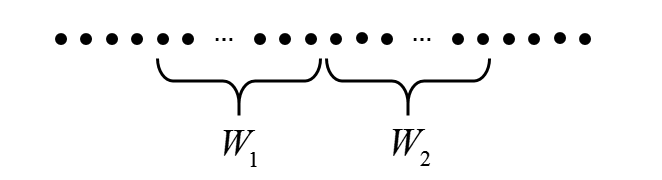
\includegraphics[width=0.4\textwidth]{img/sync_sliding_window.png}
				\caption{帧同步时滑动窗口示意图}
				\label{fig:sync_sliding_window}
			\end{figure}

			\begin{figure}
				\centering
				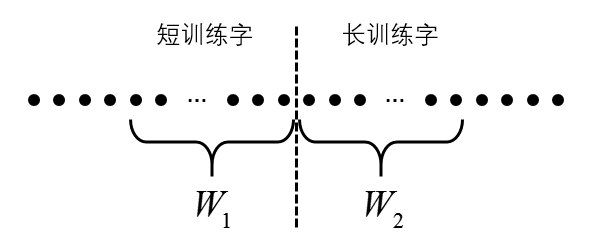
\includegraphics[width=0.4\textwidth]{img/sync_sliding_window_lts.png}
				\caption{符号同步时滑动窗口示意图}
				\label{fig:sync_sliding_window_lts}
			\end{figure}

		下面介绍如何添加同步相关性的软件接口,以互相关性为例介绍,自相关性与之类似。

		第一步,列出同步互相关性的公式,分析哪些计算适合由硬件完成,哪些计算适合引出到软件由软件完成。
		\ref{math:sync_inter_correlation}是互相关性的公式,其中$P_n$是归一化系数。
			\begin{equation}
				\centering
				C_n = \sum_{k=0}^{L-1} r_{n+k} \cdot s_{n+k}^*
			\end{equation}
			\begin{equation}
				\centering
				P_n = \sum_{k=0}^{L-1} |r_{n+k}|^2 \cdot \sum_{k=0}^{L-1} |s_{n+k}|^2
			\end{equation}
			\begin{equation}
				\centering
				M_n = \frac{|C_n|^2}{P_n}
				\label{math:sync_inter_correlation}
			\end{equation}

		我们知道FPGA硬件适合做乘法与加法,不适合做除法,除法需要多周期,延迟高。因此,我们可以把计算$C_n$与$P_n$交由硬件完成。
		另外,因为长训练字的能量值$\sum_{k=0}^{L-1} |s_{n+k}|^2$是固定的,我们只需在硬件中计算$\sum_{k=0}^{L-1} |r_{n+k}|^2$,称作$P'_n$,
		计算$M_n$的过程由软件完成。

		第二步,在同步模块内计算得到$C_n$、$P'_n$,并从同步模块引出。
		添加同步模块的端口,如下所示,这里只是示意代码,实际上除了$C_n$、$P'_n$外,我们还引出了计算自相关性的几个信号。
		\begin{lstlisting}[language={Verilog}]
module rx_synchronization(
	... // other ports
	input signal_valid,
	output [31:0] sync_para_C,
	output [31:0] sync_para_P1,
	... // other ports
);
		\end{lstlisting}
		signal\_valid信号是指后续模块解出了signal字段,只有signal字段符合要求时此值为1,否则为0。
		我们在signal\_valid为1时为sync\_para\_C、sync\_para\_P1赋值。

		第三步,做时钟域转换,把同步模块对应时钟域下的sync\_para\_C、sync\_para\_P1,
		转化为AXI总线时钟域下的axi\_sync\_para\_C、axi\_sync\_para\_P1,并赋值给AXI寄存器。
		GRTSEC提供了一个时钟域转换模块reg\_clk\_domain\_switch,使用方法如下所示,我们将$C_n$、$P'_n$合并后一起转时钟。
		\begin{lstlisting}[language={Verilog}]
reg_clk_domain_switch_64 SEC_SYNC_clk_switch_clk0_to_clkaxi(
	.clk_pre(usr_clk_ch0),
	.clk_pos(S_AXI_ACLK),
	.rst_pre(usr_rst_ch0),
	.rst_pos(~S_AXI_ARESETN),
	.reg_pre(sync_para),
	.reg_pos(axi_sync_para)
);
		\end{lstlisting}

		第四步,从嵌入式软件代码读取$C_n$、$P'_n$,并用软件计算出我们所需的$M_n$。
		嵌入式软件读取和计算代码如下所示,SYNC\_PARA\_LTS为预存好的长训练字的能量值。
		\begin{lstlisting}[language={C}]
int syncParaC = Xil_In32(PHYSyncPara1);
int syncParaP1 = Xil_In32(PHYSyncPara2);
float syncParaM = syncParaC * syncParaC / (syncParaP1 * SYNC_PARA_LTS);
		\end{lstlisting}

		至此,以同步相关性为例,用户完成了物理层信息的扩展。

		\subsection{多射频模式}\label{subsec:grtsec_loopback}
		本文在第五章设计了多个物理层WiFi安全的使用样例,使用GRTSEC进行验证,
		在实际研究过程中我们发现,在真正通过空气进行通信之前,我们需要对完美信道进行模拟。
		完美信道是指将发送端和接收端之间连接在一起,接收到的信号与发送信号完全相同,
		用以验证物理层信息是否是完美信息,比如CSI全部为1,频偏为0,同步相关性为1等,
		以及模拟在完美通信时新数据处理算法是否可行,排除信号偏差带来的影响,
		比如验证加密解密算法在硬件上运行是否正确,不需要真正地与射频前端连接起来。

		为了支持完美信道,我们对射频通信库进行了扩展,提供两种模式,射频模式和回环模式。
		射频模式是原射频通信库采用的方式,与射频前端相连。回环模式是将发送数据直接反馈给接收端。
		回环模式的示意见图\ref{fig:rflib_loopback_mux},我们将发送端FIFO的输出,直接接到了接收端FIFO的输入上。
		值得注意的是,除了数据流需要做多路选择,时钟和复位信号也要做多路选择。
		收发FIFO都是异步FIFO,在射频模式时,射频端的时钟和复位信号来自射频模块,在回环模式时,需要改成物理层时钟,
		如下所示。
		\begin{lstlisting}[language={Verilog}]
assign clk = (MODE == RFD_MODE_LOOPBACK)? PHY_clk : rf_clk;
assign rst = (MODE == RFD_MODE_LOOPBACK)? PHY_rst : rf_rst;
		\end{lstlisting}

			\begin{figure}
				\centering
				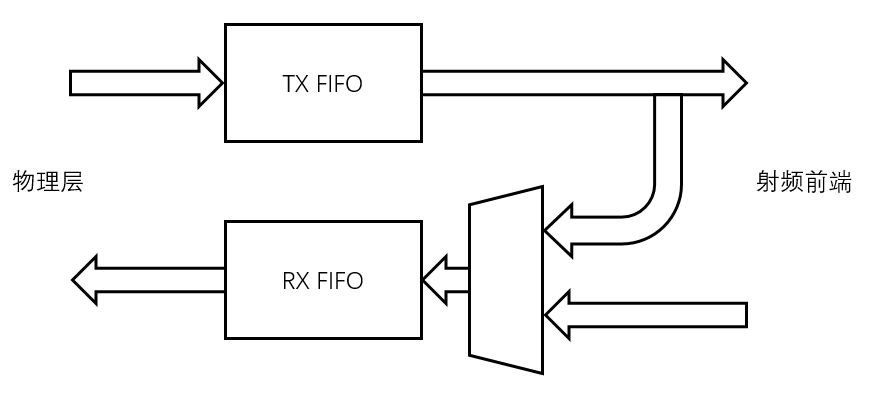
\includegraphics[width=0.7\textwidth]{img/rflib_loopback_mux.png}
				\caption{射频通信库射频模式与回环模式示意图}
				\label{fig:rflib_loopback_mux}
			\end{figure}

		回环模式在研究前期是经常用到的,在真正通过空气测试之前,研究者往往会先验证数据处理流程是否能在硬件上正常工作,
		类似于将射频前端的发送端与接收端通过馈线相连,回环模式可以替代馈线。
		另外,对于手中已有FPGA开发板,但暂时不想购买射频前端的用户来说,可以先用回环模式进行验证,可以得到一些测试结果,
		购买射频前端后,只需要修改一个参数,就能迅速适配射频前端。

		\subsection{本节小结}\label{subsec:grt2.0_summary}
		本节介绍了GRTSEC在GRT2.0系统上的改进,
		首先在\ref{subsec:grtsec_overview}小节介绍了总体设计,
		GRTSEC最核心的改进是对物理层信息进行了支持,提取了物理层信息并提供了物理层信息的编程接口,
		\ref{subsec:grtsec_phyinfo_substract}小节介绍了CSI、频偏、RSSI、调制方式的提取方法,
		\ref{subsec:grtsec_phyinfo_api}小节、\ref{subsec:grtsec_phyinfo_analyzer}小节分别介绍了物理层信息的软件和硬件接口,
		\ref{subsec:grtsec_phyinfo_extension}小节以同步相关性为例介绍了用户如何扩展物理层信息,
		\ref{subsec:grtsec_loopback}小节介绍了为提高开发调试的效率,射频通信库模块对完美信道和历史信道的支持。
